\documentclass{standalone}
\usepackage{tikz}
\usetikzlibrary{patterns, positioning}
\usepackage[sfdefault]{ClearSans} %% option 'sfdefault' activates Clear Sans as the default text font
\usepackage[T1]{fontenc}

\begin{document}
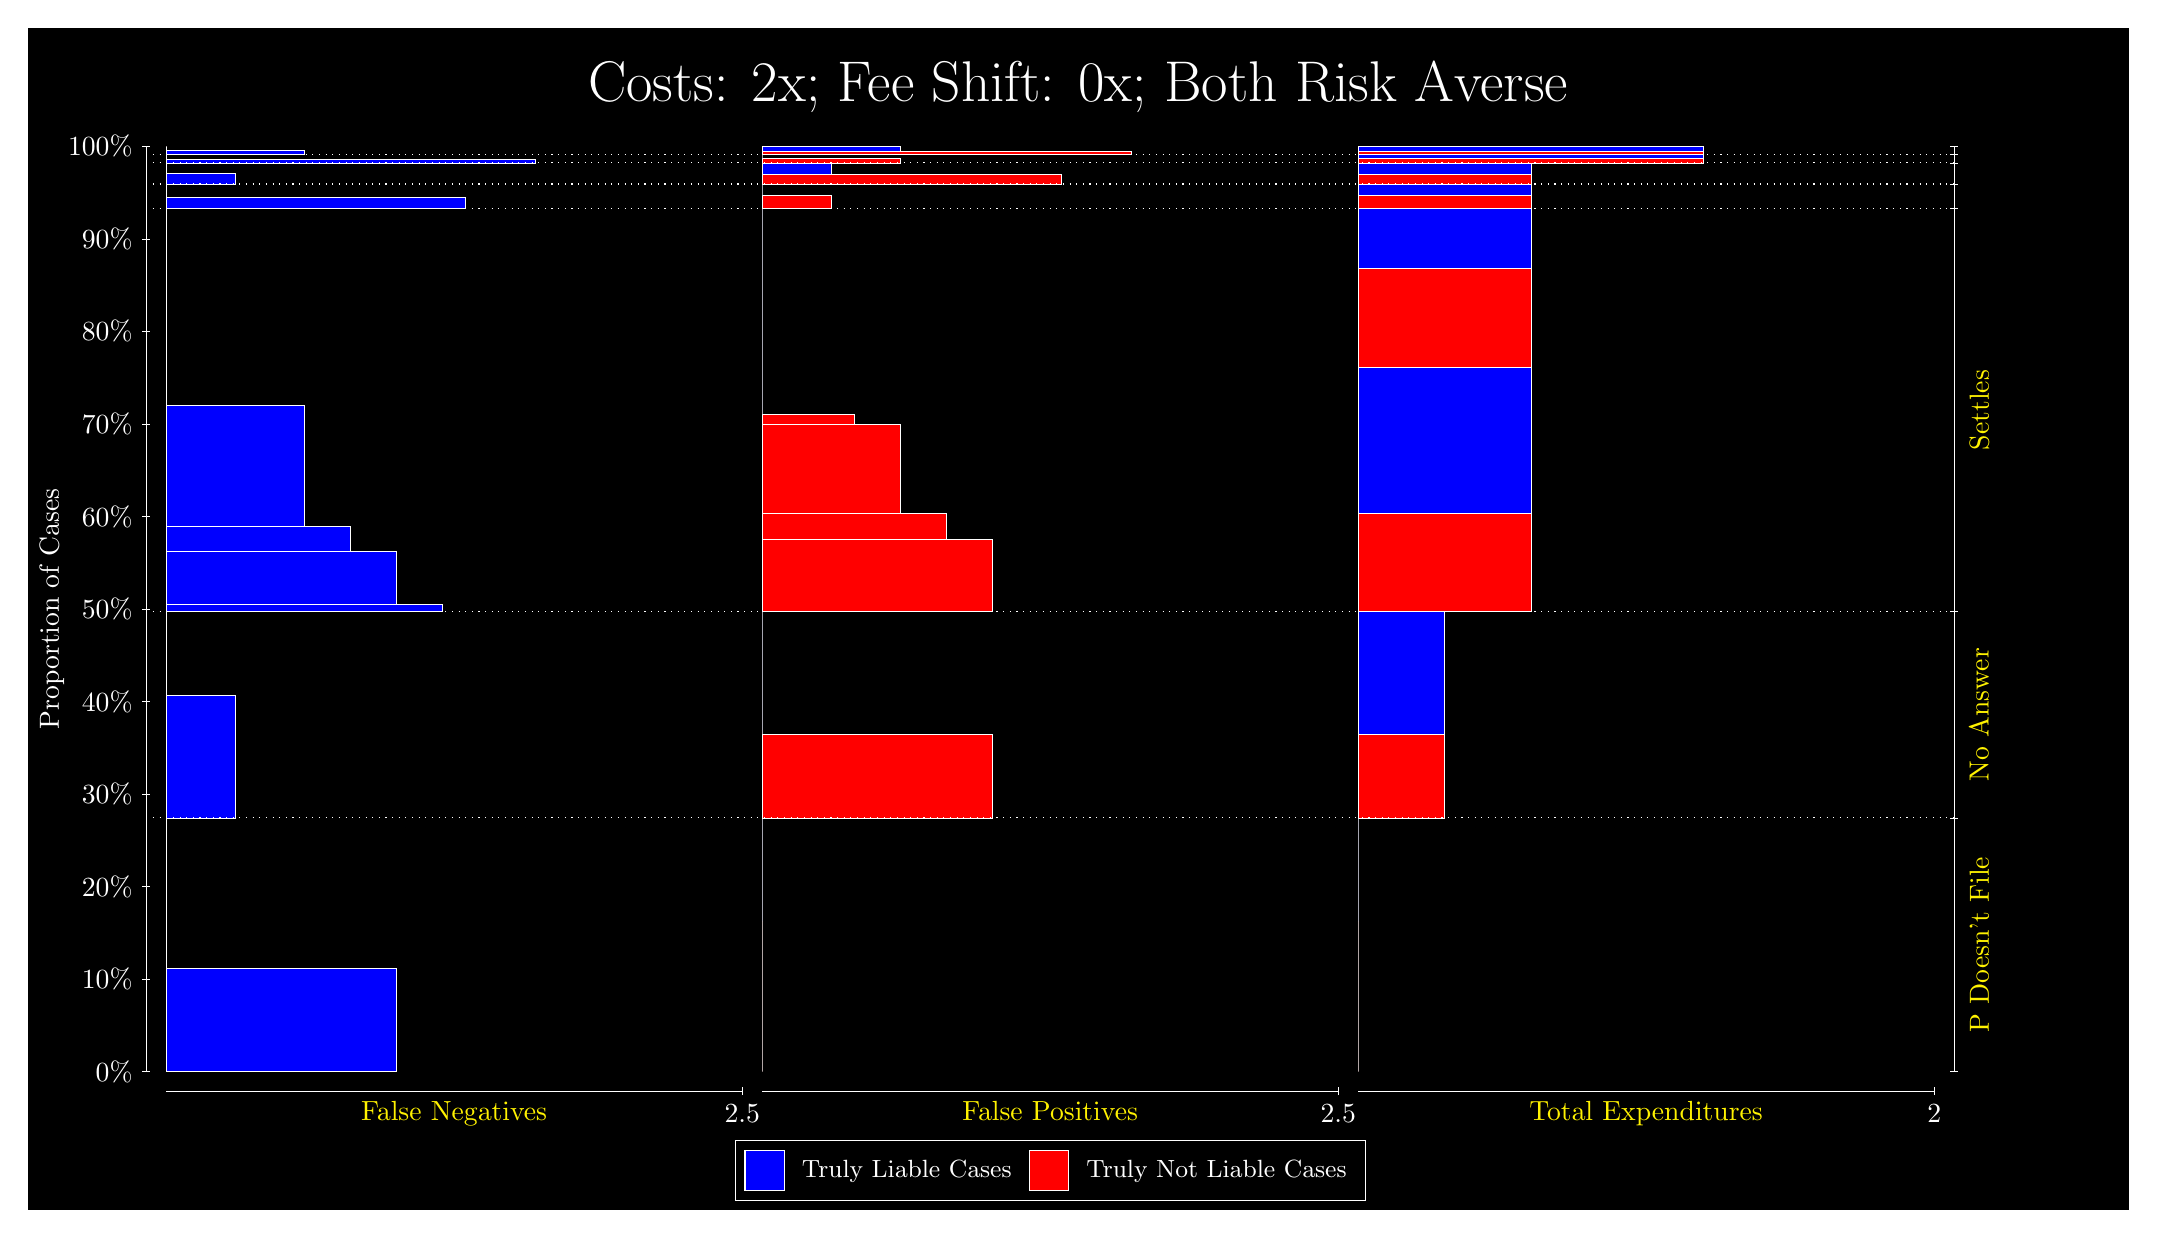
\begin{tikzpicture}
\draw[fill=black] (0,0) rectangle (26.667,15);
\draw[text=white] (0,13.5) rectangle (26.667,15) node[midway] {\huge Costs: 2x; Fee Shift: 0x; Both Risk Averse};
\draw[white, very thin] (1.5,1.75) -- (1.5,13.5);
\node[rotate=90, text=white, anchor=center] at (0.3, 7.625) {Proportion of Cases};
\draw[white, very thin] (1.45,1.75) -- (1.55,1.75);
\node[text=white, anchor=east] at (1.45, 1.75) {0\%};
\draw[white, very thin] (1.45,2.925) -- (1.55,2.925);
\node[text=white, anchor=east] at (1.45, 2.925) {10\%};
\draw[white, very thin] (1.45,4.1) -- (1.55,4.1);
\node[text=white, anchor=east] at (1.45, 4.1) {20\%};
\draw[white, very thin] (1.45,5.275) -- (1.55,5.275);
\node[text=white, anchor=east] at (1.45, 5.275) {30\%};
\draw[white, very thin] (1.45,6.45) -- (1.55,6.45);
\node[text=white, anchor=east] at (1.45, 6.45) {40\%};
\draw[white, very thin] (1.45,7.625) -- (1.55,7.625);
\node[text=white, anchor=east] at (1.45, 7.625) {50\%};
\draw[white, very thin] (1.45,8.8) -- (1.55,8.8);
\node[text=white, anchor=east] at (1.45, 8.8) {60\%};
\draw[white, very thin] (1.45,9.975) -- (1.55,9.975);
\node[text=white, anchor=east] at (1.45, 9.975) {70\%};
\draw[white, very thin] (1.45,11.15) -- (1.55,11.15);
\node[text=white, anchor=east] at (1.45, 11.15) {80\%};
\draw[white, very thin] (1.45,12.325) -- (1.55,12.325);
\node[text=white, anchor=east] at (1.45, 12.325) {90\%};
\draw[white, very thin] (1.45,13.5) -- (1.55,13.5);
\node[text=white, anchor=east] at (1.45, 13.5) {100\%};

\draw[white, very thin] (24.457,1.75) -- (24.457,13.5);
\draw[white, very thin] (24.407,1.75) -- (24.507,1.75);
\node[anchor=west] at (24.407, 1.75) {};
\draw[white, very thin] (24.407,4.9712) -- (24.507,4.9712);
\node[anchor=west] at (24.407, 4.9712) {};
\draw[white, very thin] (24.407,7.5937) -- (24.507,7.5937);
\node[anchor=west] at (24.407, 7.5937) {};
\draw[white, very thin] (24.407,12.709) -- (24.507,12.709);
\node[anchor=west] at (24.407, 12.709) {};
\draw[white, very thin] (24.407,13.021) -- (24.507,13.021);
\node[anchor=west] at (24.407, 13.021) {};
\draw[white, very thin] (24.407,13.289) -- (24.507,13.289);
\node[anchor=west] at (24.407, 13.289) {};
\draw[white, very thin] (24.407,13.395) -- (24.507,13.395);
\node[anchor=west] at (24.407, 13.395) {};
\draw[white, very thin] (24.407,13.5) -- (24.507,13.5);
\node[anchor=west] at (24.407, 13.5) {};

\draw[white, very thin, fill=blue] (1.75,1.75) rectangle (4.6775,3.0608);
\draw[white, very thin, fill=red] (1.75,3.0608) rectangle (1.75,4.9712);
\draw[white, very thin, fill=blue] (1.75,4.9712) rectangle (2.6283,6.5265);
\draw[white, very thin, fill=red] (1.75,6.5265) rectangle (1.75,7.5937);
\draw[white, very thin, fill=blue] (1.75,7.5937) rectangle (5.2631,7.6805);
\draw[white, very thin, fill=blue] (1.75,7.6805) rectangle (4.9703,7.6826);
\draw[white, very thin, fill=blue] (1.75,7.6826) rectangle (4.6775,8.3545);
\draw[white, very thin, fill=blue] (1.75,8.3545) rectangle (4.092,8.6778);
\draw[white, very thin, fill=blue] (1.75,8.6778) rectangle (3.5065,10.212);
\draw[white, very thin, fill=red] (1.75,10.212) rectangle (1.75,12.709);
\draw[white, very thin, fill=blue] (1.75,12.709) rectangle (5.5558,12.857);
\draw[white, very thin, fill=red] (1.75,12.857) rectangle (1.75,13.021);
\draw[white, very thin, fill=blue] (1.75,13.021) rectangle (2.6283,13.159);
\draw[white, very thin, fill=red] (1.75,13.159) rectangle (1.75,13.289);
\draw[white, very thin, fill=blue] (1.75,13.289) rectangle (6.4341,13.336);
\draw[white, very thin, fill=red] (1.75,13.336) rectangle (1.75,13.395);
\draw[white, very thin, fill=blue] (1.75,13.395) rectangle (3.5065,13.453);
\draw[white, very thin, fill=red] (1.75,13.453) rectangle (1.75,13.5);
\draw[white, very thin, fill=red] (9.3189,1.75) rectangle (9.3189,3.6605);
\draw[white, very thin, fill=blue] (9.3189,3.6605) rectangle (9.3189,4.9712);
\draw[white, very thin, fill=red] (9.3189,4.9712) rectangle (12.246,6.0384);
\draw[white, very thin, fill=blue] (9.3189,6.0384) rectangle (9.3189,7.5937);
\draw[white, very thin, fill=red] (9.3189,7.5937) rectangle (12.246,8.5156);
\draw[white, very thin, fill=red] (9.3189,8.5156) rectangle (11.661,8.8417);
\draw[white, very thin, fill=red] (9.3189,8.8417) rectangle (11.075,9.967);
\draw[white, very thin, fill=red] (9.3189,9.967) rectangle (10.783,9.9699);
\draw[white, very thin, fill=red] (9.3189,9.9699) rectangle (10.49,10.091);
\draw[white, very thin, fill=blue] (9.3189,10.091) rectangle (9.3189,12.709);
\draw[white, very thin, fill=red] (9.3189,12.709) rectangle (10.197,12.873);
\draw[white, very thin, fill=blue] (9.3189,12.873) rectangle (9.3189,13.021);
\draw[white, very thin, fill=red] (9.3189,13.021) rectangle (13.125,13.151);
\draw[white, very thin, fill=blue] (9.3189,13.151) rectangle (10.197,13.289);
\draw[white, very thin, fill=red] (9.3189,13.289) rectangle (11.075,13.348);
\draw[white, very thin, fill=blue] (9.3189,13.348) rectangle (9.3189,13.395);
\draw[white, very thin, fill=red] (9.3189,13.395) rectangle (14.003,13.441);
\draw[white, very thin, fill=blue] (9.3189,13.441) rectangle (11.075,13.5);
\draw[white, very thin, fill=red] (16.888,1.75) rectangle (16.888,3.6605);
\draw[white, very thin, fill=blue] (16.888,3.6605) rectangle (16.888,4.9712);
\draw[white, very thin, fill=red] (16.888,4.9712) rectangle (17.986,6.0384);
\draw[white, very thin, fill=blue] (16.888,6.0384) rectangle (17.986,7.5937);
\draw[white, very thin, fill=red] (16.888,7.5937) rectangle (19.083,8.8417);
\draw[white, very thin, fill=blue] (16.888,8.8417) rectangle (19.083,10.699);
\draw[white, very thin, fill=red] (16.888,10.699) rectangle (19.083,11.948);
\draw[white, very thin, fill=blue] (16.888,11.948) rectangle (19.083,12.709);
\draw[white, very thin, fill=red] (16.888,12.709) rectangle (19.083,12.873);
\draw[white, very thin, fill=blue] (16.888,12.873) rectangle (19.083,13.021);
\draw[white, very thin, fill=red] (16.888,13.021) rectangle (19.083,13.151);
\draw[white, very thin, fill=blue] (16.888,13.151) rectangle (19.083,13.289);
\draw[white, very thin, fill=red] (16.888,13.289) rectangle (21.279,13.348);
\draw[white, very thin, fill=blue] (16.888,13.348) rectangle (21.279,13.395);
\draw[white, very thin, fill=red] (16.888,13.395) rectangle (21.279,13.441);
\draw[white, very thin, fill=blue] (16.888,13.441) rectangle (21.279,13.5);
\draw[white, dotted] (1.5,4.9712) -- (24.457,4.9712);
\draw[white, dotted] (1.5,7.5937) -- (24.457,7.5937);
\draw[white, dotted] (1.5,12.709) -- (24.457,12.709);
\draw[white, dotted] (1.5,13.021) -- (24.457,13.021);
\draw[white, dotted] (1.5,13.289) -- (24.457,13.289);
\draw[white, dotted] (1.5,13.395) -- (24.457,13.395);
\draw[white, very thin] (1.75,1.5) -- (9.0689,1.5);
\node[text=yellow, anchor=north] at (5.4094, 1.5) {False Negatives};
\draw[white, very thin] (9.0689,1.45) -- (9.0689,1.55);
\node[text=white, anchor=north] at (9.0689, 1.45) {2.5};

\draw[white, very thin] (9.3189,1.5) -- (16.638,1.5);
\node[text=yellow, anchor=north] at (12.978, 1.5) {False Positives};
\draw[white, very thin] (16.638,1.45) -- (16.638,1.55);
\node[text=white, anchor=north] at (16.638, 1.45) {2.5};

\draw[white, very thin] (16.888,1.5) -- (24.207,1.5);
\node[text=yellow, anchor=north] at (20.547, 1.5) {Total Expenditures};
\draw[white, very thin] (24.207,1.45) -- (24.207,1.55);
\node[text=white, anchor=north] at (24.207, 1.45) {2};

\node[text=yellow, centered, rotate=90] at (24.777, 3.3606) {P Doesn't File};
\node[text=yellow, centered, rotate=90] at (24.777, 6.2824) {No Answer};
\node[text=yellow, centered, rotate=90] at (24.777, 10.151) {Settles};





\draw (12.978300999999998,1.5) node[draw=none] (baseCoordinate) {};
\begin{scope}[align=center]
        \matrix[scale=0.5, draw=white, below=0.5cm of baseCoordinate, nodes={draw}, column sep=0.1cm]{
            \node[rectangle, draw, minimum width=0.5cm, minimum height=0.5cm, fill=blue] {}; &
            \node[draw=none, font=\small, text=white] (B) {Truly Liable Cases}; &
            \node[rectangle, draw, minimum width=0.5cm, minimum height=0.5cm, fill=red] {}; &
            \node[draw=none, font=\small, text=white] (B) {Truly Not Liable Cases}; \\
            };
\end{scope}

\end{tikzpicture}
\end{document}